\chapter{Reinforcement Learning Approach}
\section{Introduction}
\section{Reinforcement Learning}
\subsection{Definition}
\citeauthor{RLIntroduction} \cite[Chapter.~1]{RLIntroduction} gave an excellent in-depth definition, which not only defines what RL is, but also compare it with other ML methods.
\newline We will summarize it as follow:
\begin{definition}
	RL deals with opti
\end{definition}
\begin{figure}
	\centering
	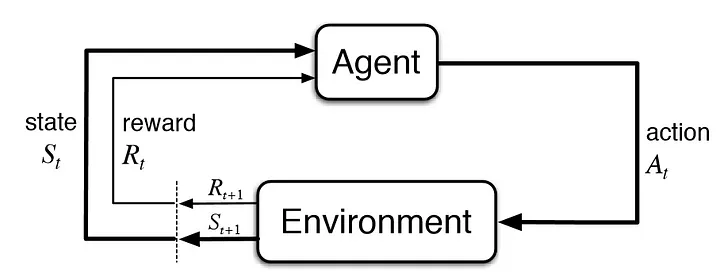
\includegraphics[width= 0.8\textwidth]{Figures/RLDiagram.png}
	\caption{A Reinforcement Learning system}
\end{figure}
\subsection{Single Agent}
In most settings, the theory of reinforcement learning deals with environments where we would like to optimize a single agent. This is called single-agent reinforcement learning. This is usually modeled with a Markov Decision Process \cite[Chapter~3]{RLIntroduction}.
\newline Reinforcement Learning methods differ by their underlying assumptions

\subsection{Multi Agent}
In our case, a Mean Payoff Game can be modelled in the reinforcement learning setting as a Stochastic Game\footnote{Also known as Markov Game} \cite{StochasticGames}.
\newline This is a powerfull tool, as it can also model the stochastic version of mean payoff games \cite{StochasticMPG}. 

\subsection{Markov Chains}
\subsection{Markov Reward Process}
\section{Monte Carlo Augmentation}
\subsection{Monte Carlo Tree Search}
Monte Carlo Tree Search (MCTS) is a crucial algorith \cite{MCTS}
\section{Services}
\section{Pipeline}
\begin{figure}
	\centering
	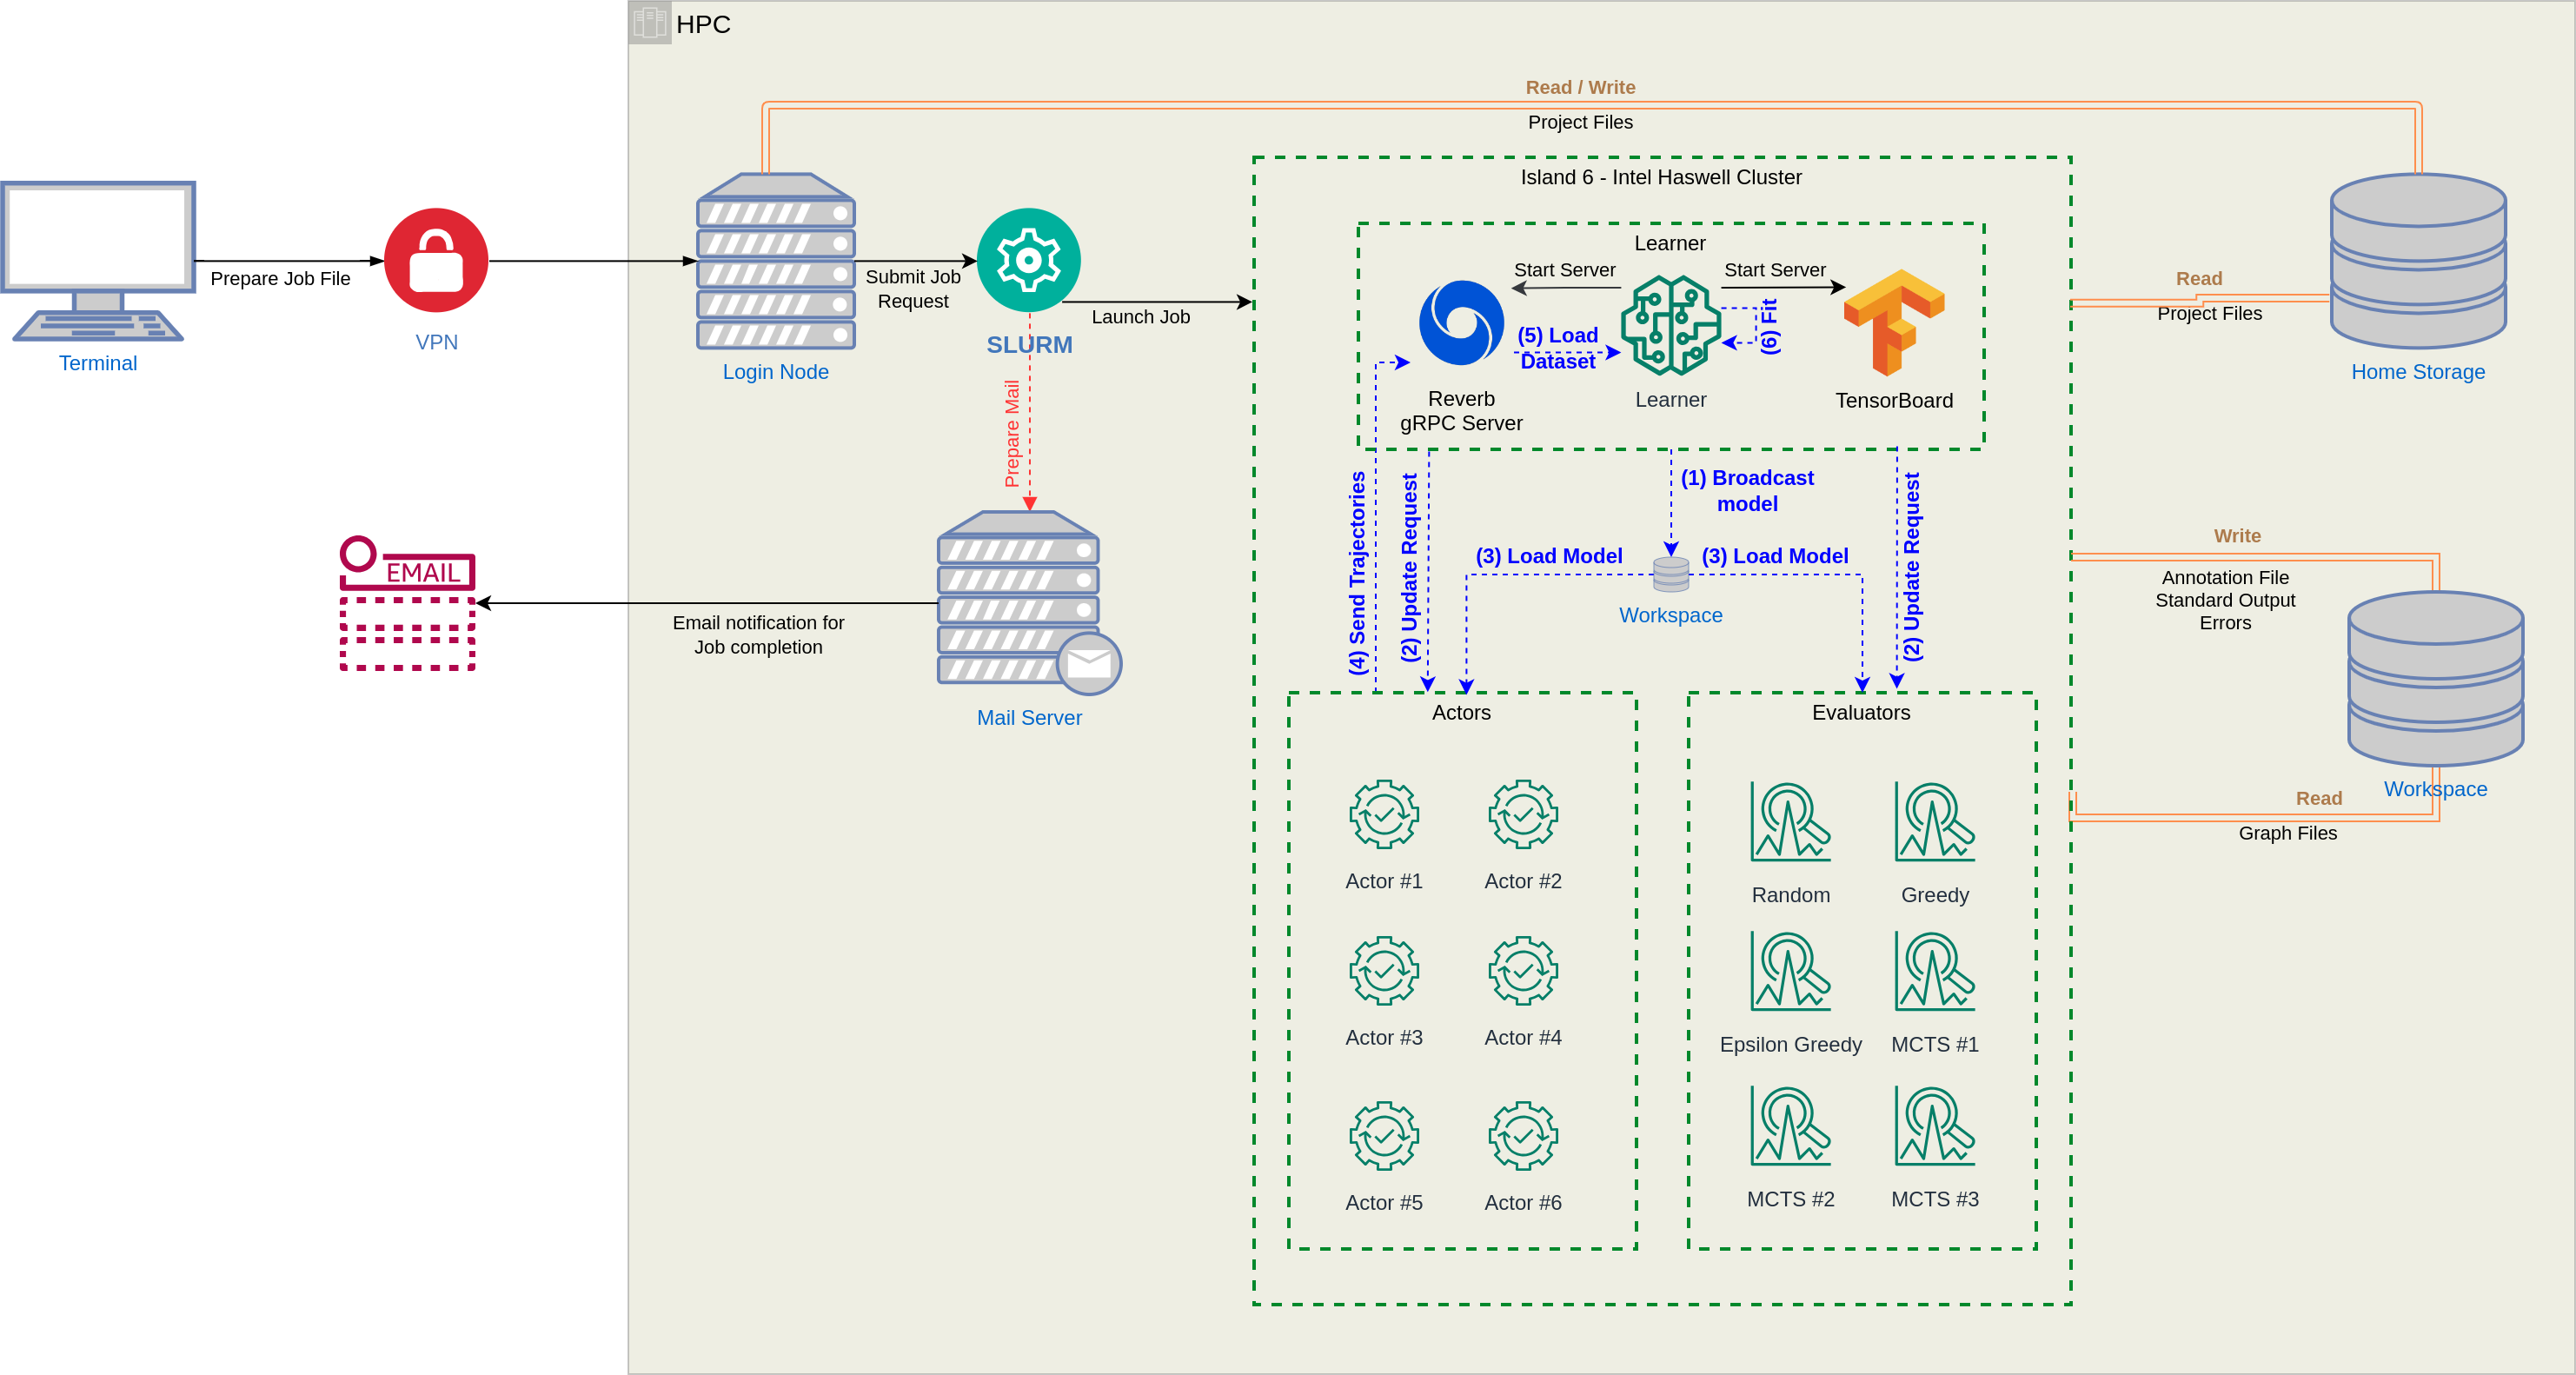
\includegraphics[width=0.95\textwidth]{Figures/AlphaZero.png}
	\caption{Pipeline Architecture}
\end{figure}
\section{Configuration}
